\documentclass{article}

\usepackage{amsmath}
\usepackage{caption}
\usepackage{fancyhdr}
\usepackage{float}
\usepackage[a4paper, margin=1in]{geometry}
\usepackage{graphicx}
\usepackage{hyperref}
\usepackage{indentfirst}
\usepackage{wrapfig}
\usepackage{xurl}


\linespread{1.2}


\pagestyle{fancy}
\fancyhead[L]{Defense Report : \textit{Task List}}
\fancyhead[R]{
    \begin{minipage}{1.5cm}
        \centering
        
\includegraphics[width=1cm]{illustrations/icon.png}
    \end{minipage}
    }
\fancyfoot[C]{
    \begin{minipage}{1.5cm}
        \centering
        \includegraphics[width=1cm]{illustrations/EPITA.png}
    \end{minipage}
    }
\fancyfoot[R]{\thepage}


\renewcommand{\footrulewidth}{0.1pt}
\renewcommand{\sectionmark}[1]{}
\renewcommand{\subsectionmark}[1]{}
\renewcommand{\contentsname}{}


\title{\textbf{Final Defense Report}\\
\textbf{\textit{Task List}}}
\date{May 2026}
\author{
    \begin{minipage}[c]{\textwidth}
        \centering
        
\includegraphics[width=5in]{illustrations/icon.png}
    \end{minipage}
}










\begin{document}

\maketitle

\vfill
\begin{center}
    \textbf{Le Berre Adrien - A1}\\
    \textbf{Lin Jérôme - A1}\\
    \textbf{Bidault Quentin - C1}\\
    \textbf{Dupuis Alexandre - C1}\\
\end{center}






\newpage
\thispagestyle{empty}
\addtocounter{page}{-1}
\null





\newpage
\section*{Introduction}
This report presents an overview of the work carried out by the Task List team to develop an efficient task management application. It introduces the members of the group as well as their respective roles and responsibilities throughout the project.
\\

This document also describes the main features implemented to successfully build a functional and reliable task management system. It provides an analysis of the design and implementation choices, both from a technical and structural point of view, as well as the challenges encountered during the development process within a limited timeframe.





\newpage
\section*{Table of contents}
\tableofcontents





\newpage
\section{Presentation of the project}
\subsection{Members, roles and missions}
The team is composed of three active members that share a passion for computer science. With different technical experiences, each member of the group brings valuable skills to this project.

\subsubsection{Quentin Bidault}
\begin{wrapfigure}[6]{l}{0.18\textwidth}
    \vspace{-10pt}
    
\includegraphics[width=0.18\textwidth]{illustrations/members/quentin.jpg}
\end{wrapfigure}
Currently in his second year at EPITA, Quentin is a curious and determined student. He is proficient in several key programming languages (Python, Rust, C, C\#, and SQL), which he applies to his projects. In the past, he designed the assets and save system for a video game, as well as the image processing for an OCR. For this project developed in Rust, Quentin handled the sorting system and the management of recurring tasks.
\vspace{25pt}

\subsubsection{Alexandre Dupuis}
\begin{wrapfigure}{r}{0.18\textwidth}
    \vspace{-25pt}
    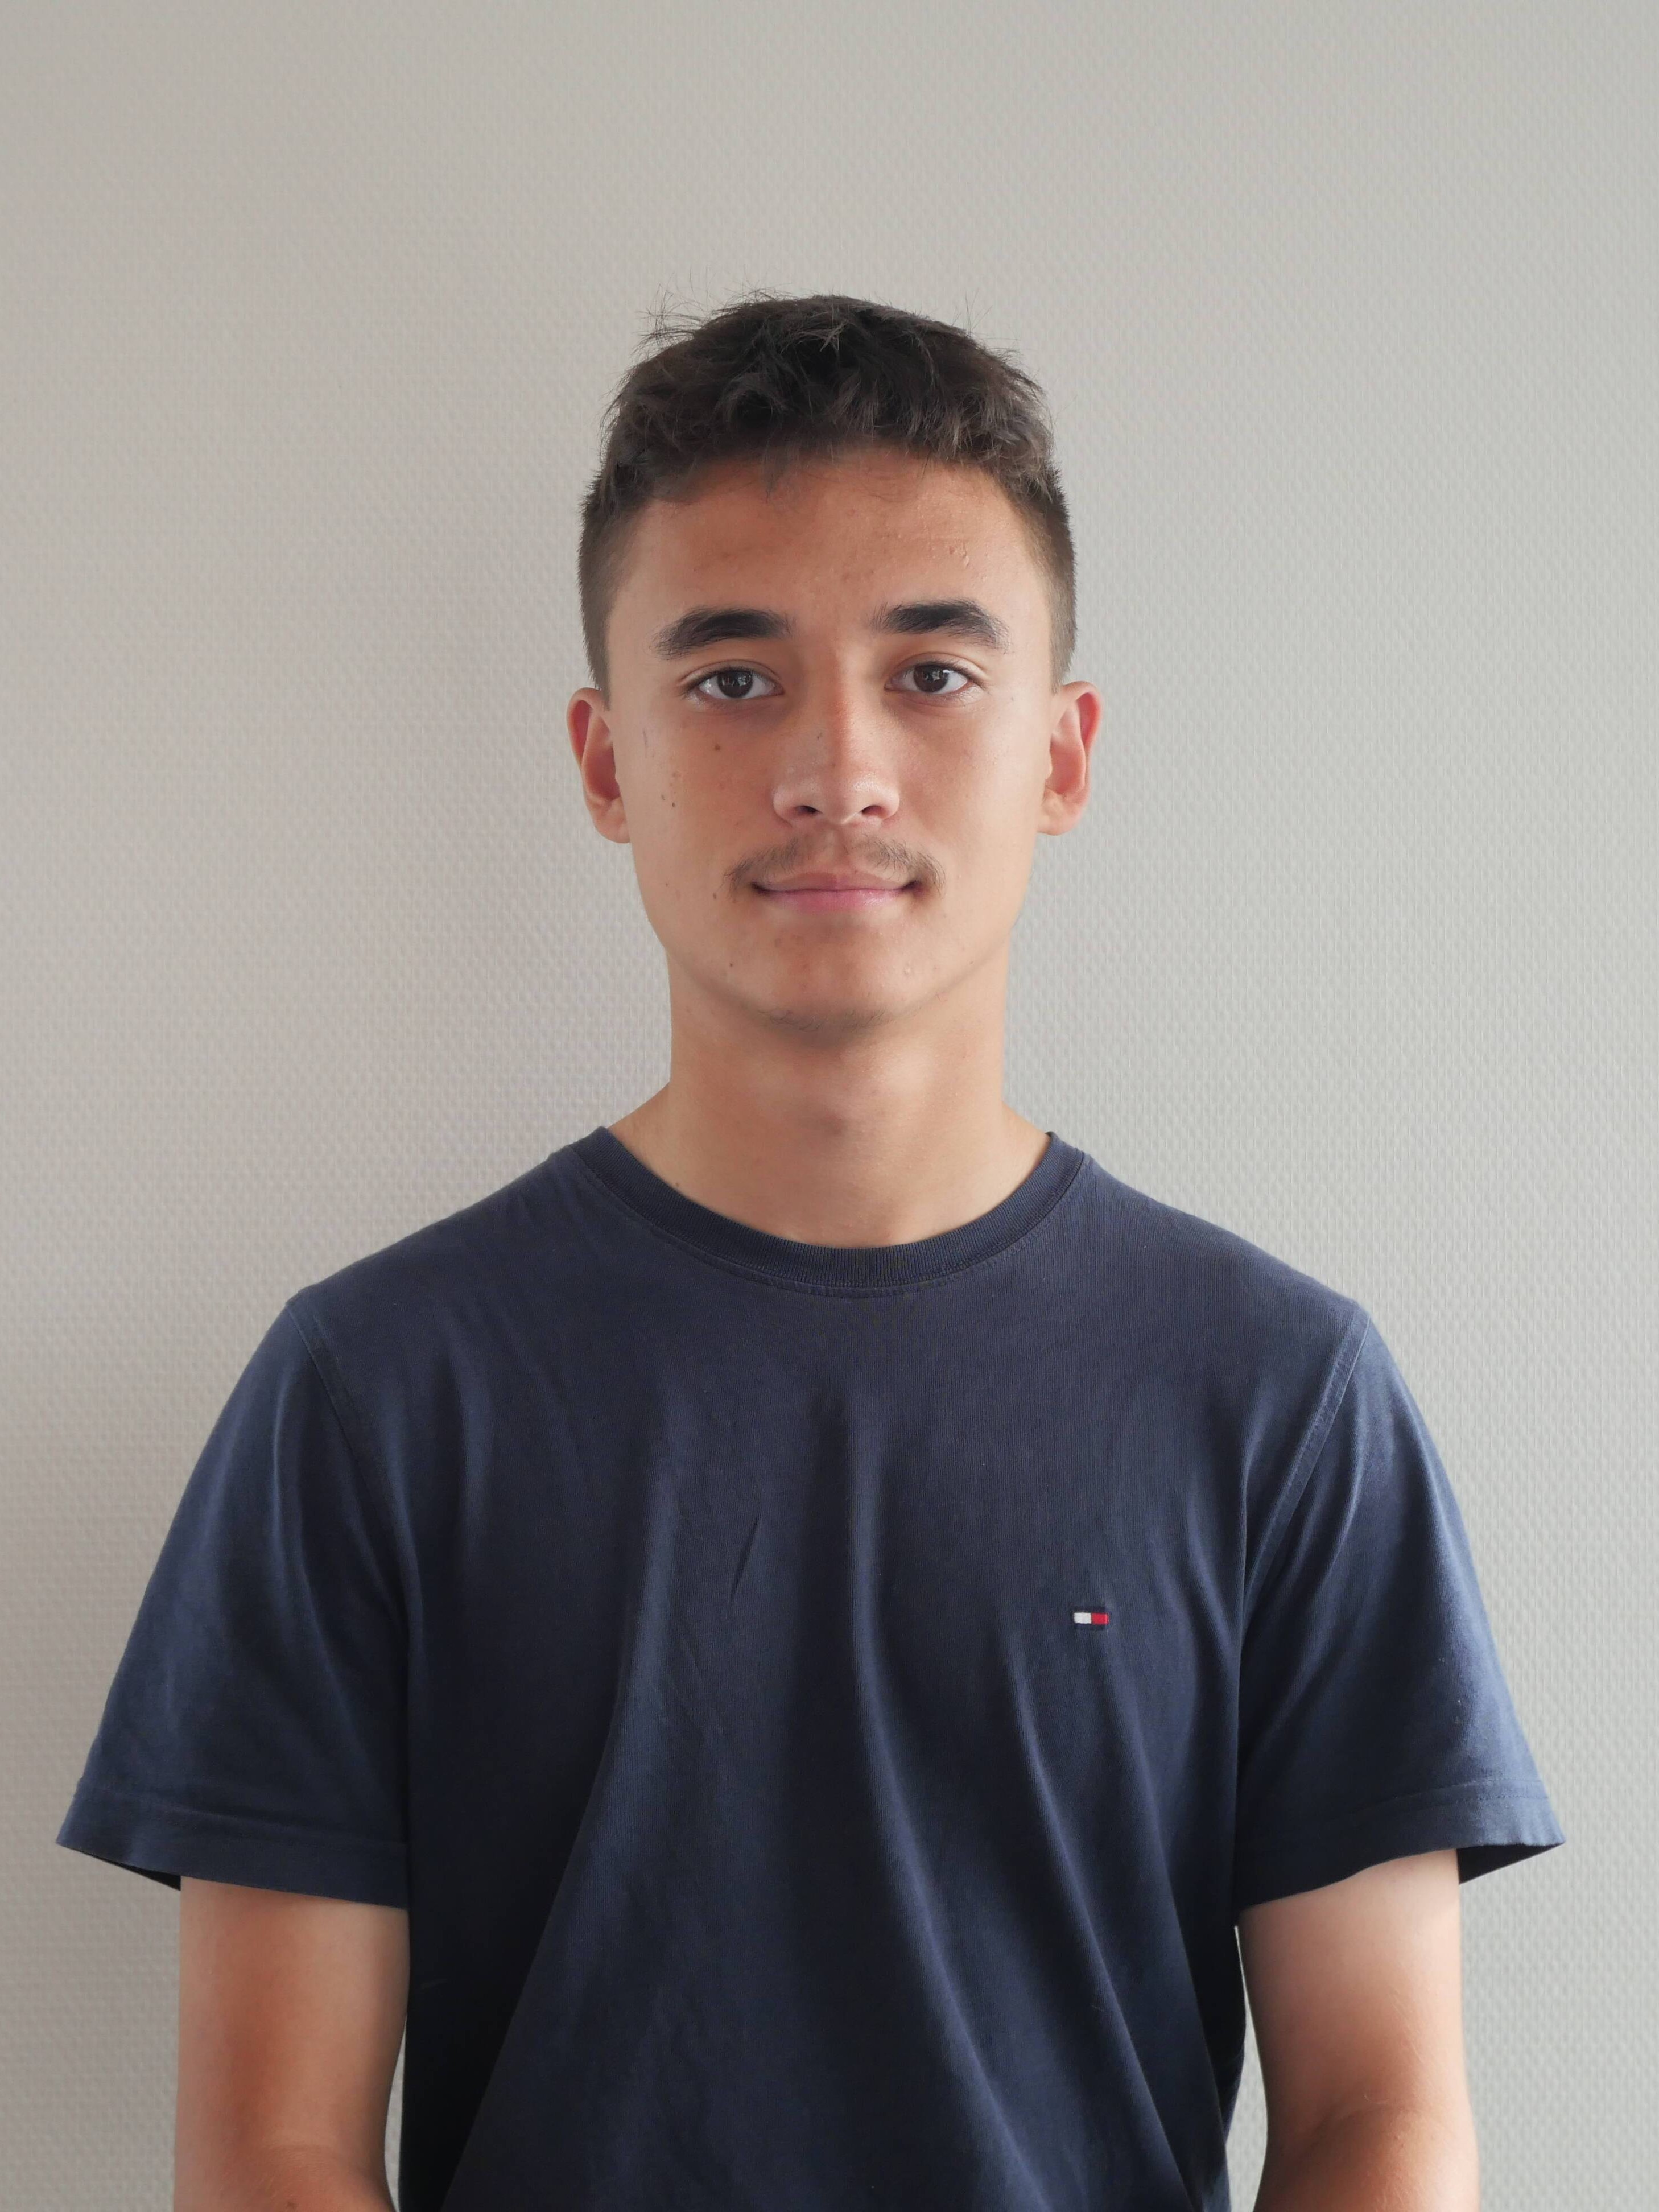
\includegraphics[width=0.18\textwidth]{illustrations/members/alexandre.jpg}
\end{wrapfigure}
Currently in his second year at EPITA, Alexandre is a serious and hardworking student. He knows several programming languages, such as C\#, C, Python, and Rust, thanks to his studies at EPITA and his past projects. When developing his previous video game, he was responsible for the music composition and the enemy system logic. He also handled element detection and image cropping for the OCR project. For this project, he is in charge of implementing the task categories, the data persistence system, and the import/export feature.

\subsubsection{Adrien Le Berre}
\begin{wrapfigure}{l}{0.18\textwidth}
    \vspace{10pt}
    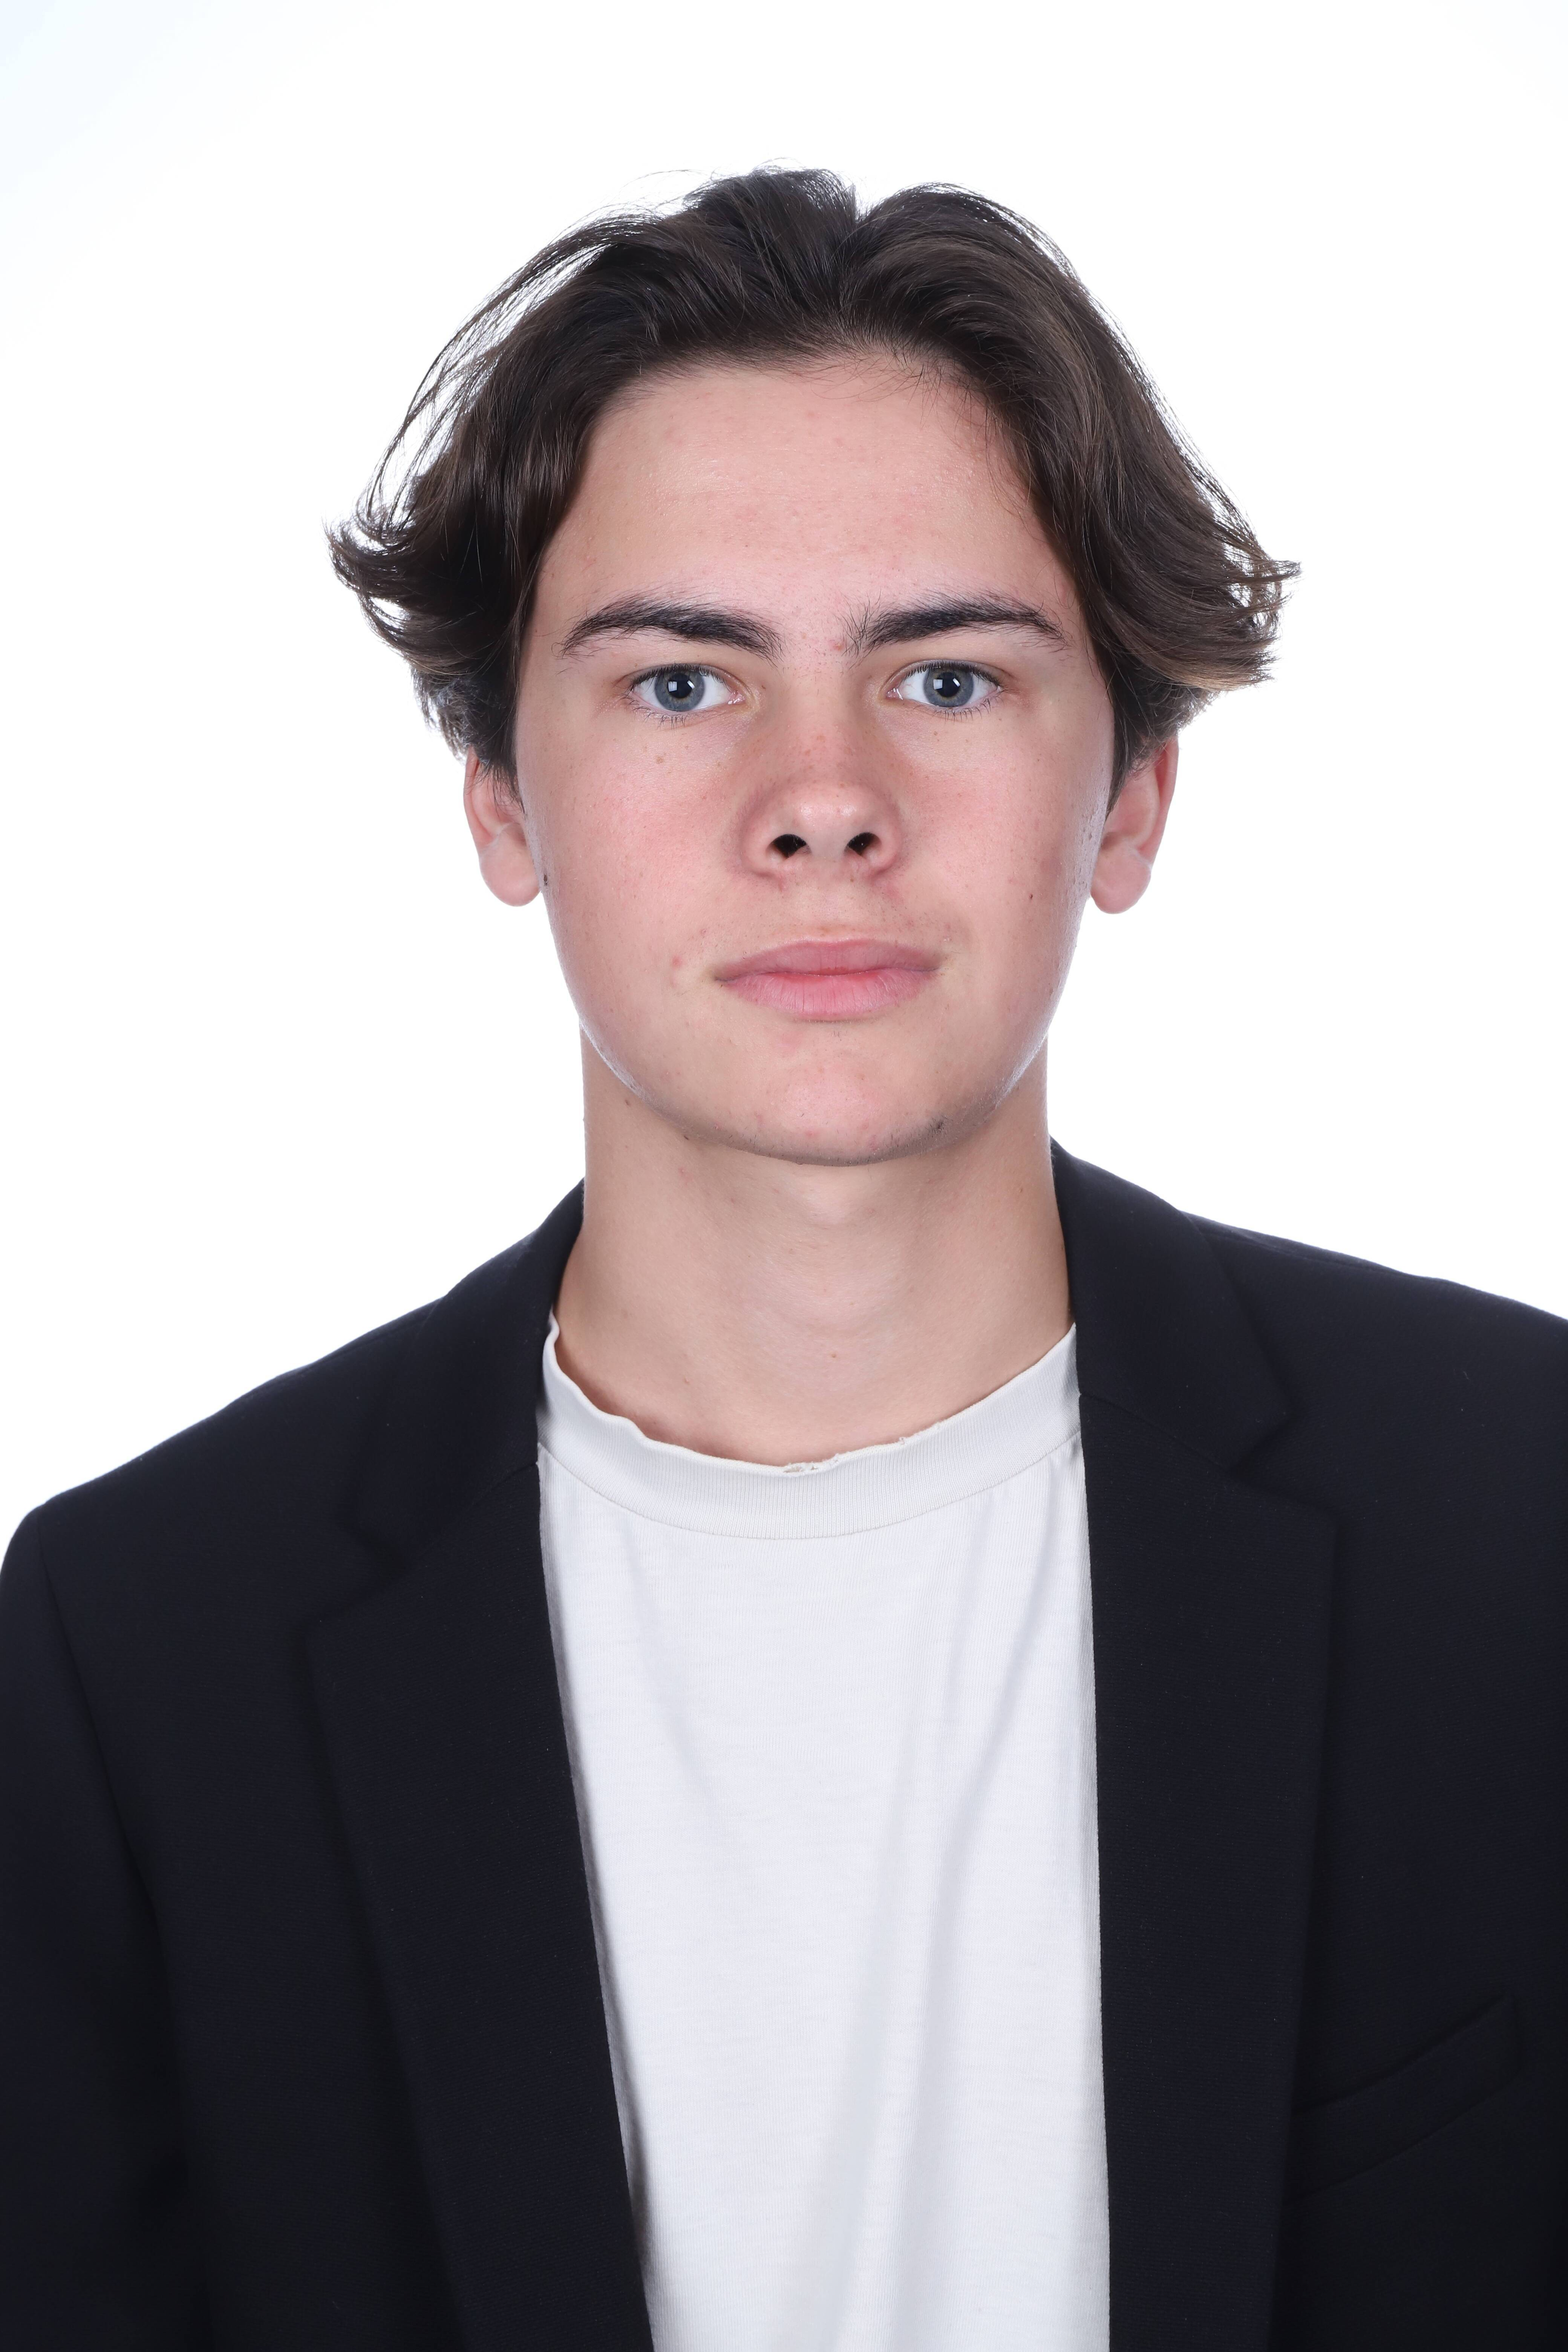
\includegraphics[width=0.18\textwidth]{illustrations/members/adrien.jpg}
\end{wrapfigure}
Currently in his second year at EPITA, Adrien Le Berre demonstrated strong rigor and adaptability throughout his academic projects. During his studies, he acquired proficiency in several programming languages, including Python, Rust, C, C\#, as well as web technologies such as HTML, CSS, and JavaScript. During his previous project such as a video game development project in which he was responsible for implementing core gameplay mechanics, ensuring the consistency and functionality of the game systems. In a separate OCR-related project, he was in charge of the user interface, focusing on usability, clarity, and overall user experience. In the current project, he was responsible for the implementation of task management within a Rust application, including the development of core task structures and basic task operations such as creation and manipulation. In addition, he designed and developed the associated website

\subsubsection{Jérôme Lin}
%\vspace{-20pt}
\begin{wrapfigure}{r}{0.18\textwidth}
    \vspace{-25pt}
    \centering
    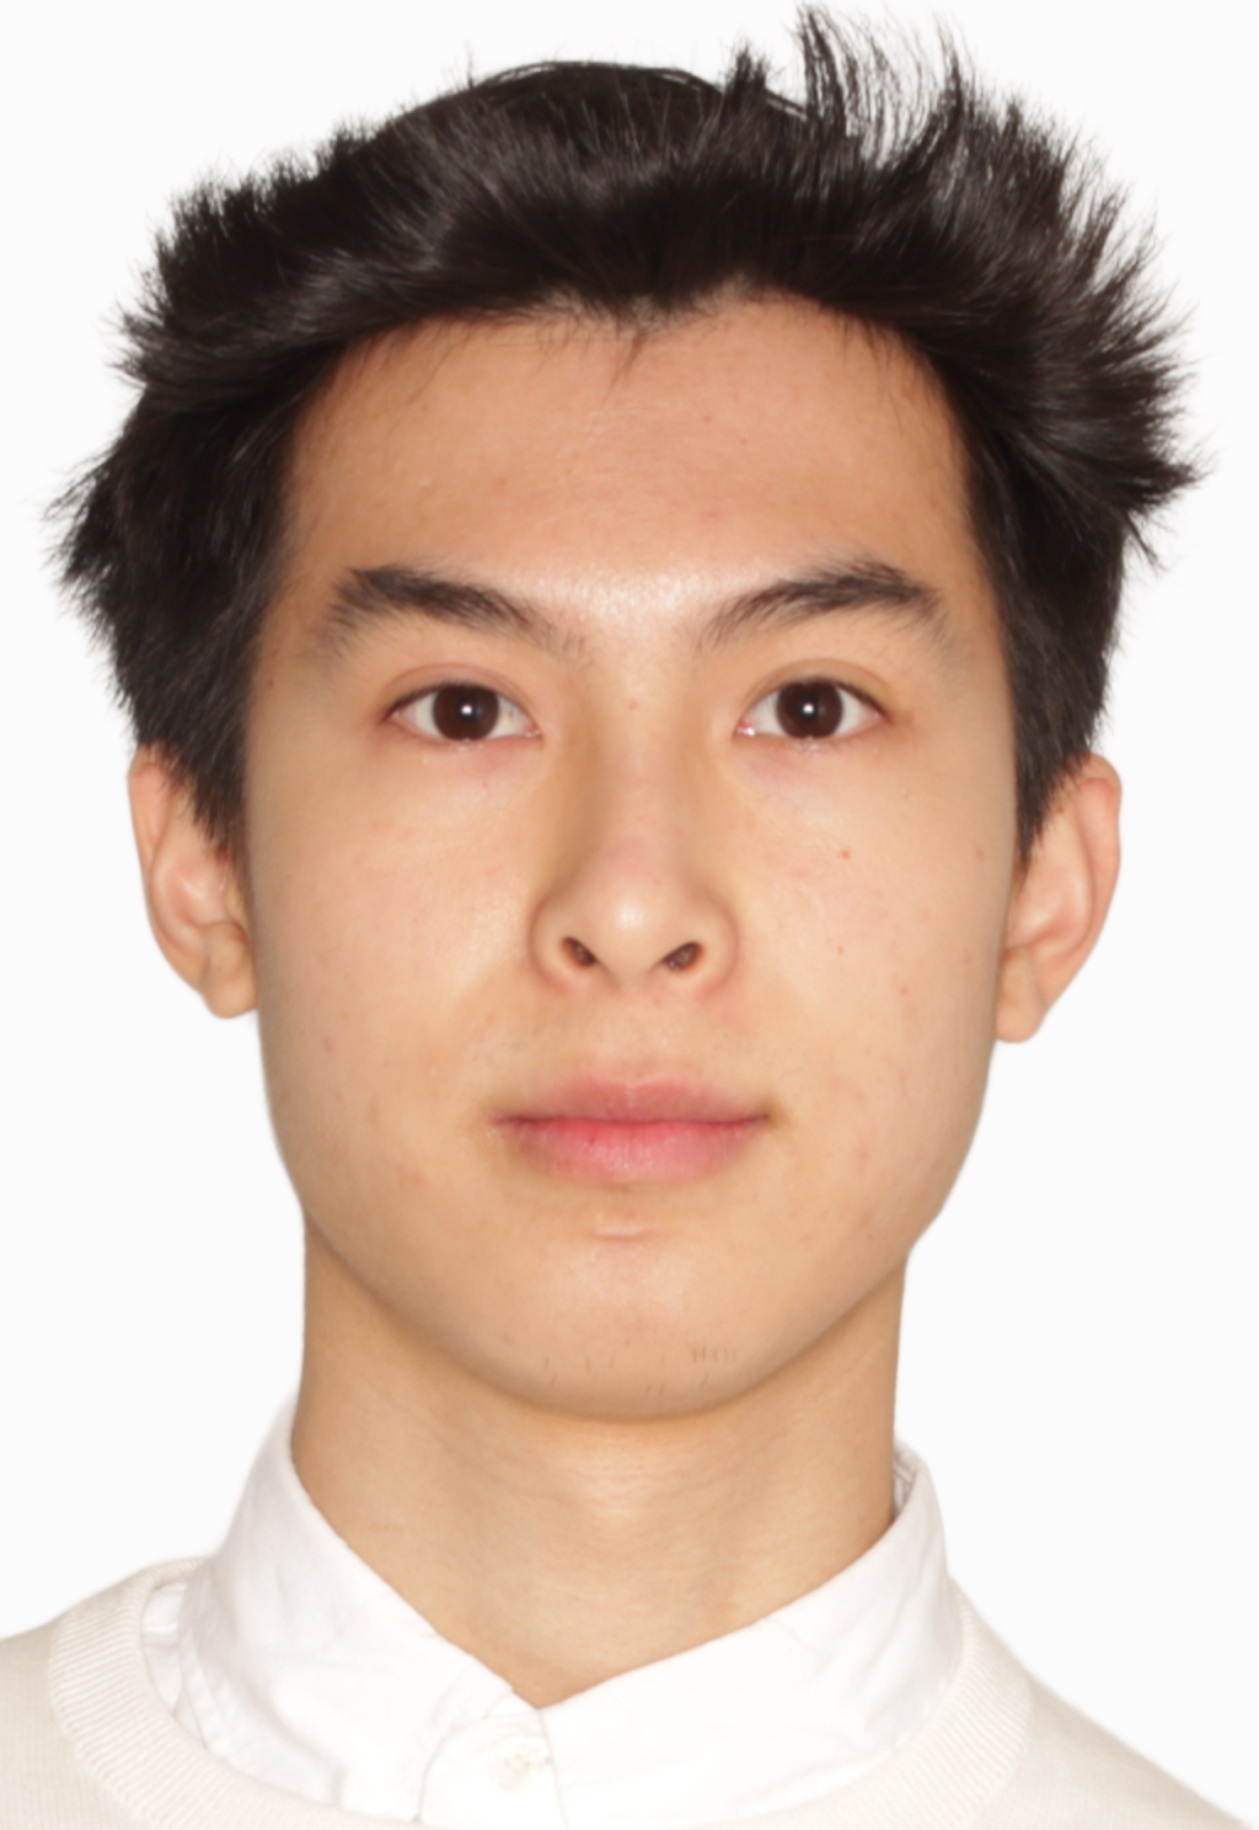
\includegraphics[width=0.18\textwidth]{illustrations/members/jerome.jpg}
\end{wrapfigure} 
Currently in his second year at EPITA, Jérôme stood out for his rigor and efficiency. During his studies, he learned several programming languages such as Python, C\#, C and Rust which he uses to design efficient and innovative solutions. During his previous video game project, he was in charge of managing the inventory system and the statistics of the items and he was also responsible of the Neural network in the previous OCR project. As the team member responsible for the user interface and the calendar view.



\newpage
\subsection{Task List project}
\subsubsection{Objective}
This project aims to build a program for handling tasks, making it possible to form, sort, manage them without difficulty. Efficiency in tracking stems from reliance solely on tools present within the institution's computer systems. With access limited to existing library resources, functionality must emerge under fixed conditions. Operation depends entirely upon what machines already provide. Design choices follow constraints set by available components.
\\

This software must save, then later retrieve, a set of tasks using an organized format like JSON so information remains intact across launches. Contained within every task: a name, explanation, current state (like pending, in progress, done), importance grade, along with deadline details. Built into its core, a resilient structure managing how tasks are added, adjusted, removed, or reordered efficiently. Structure matters most when actions shift data frequently, silently, without loss.
\\

Managing task states along with their priority levels forms part of the system's required capabilities, enabling arrangement and filtering based on various conditions. When it comes to dates, careful processing applies, especially around repeating entries tied to calendar months, with logic built in to handle irregularities like shorter months correctly.
\\

From within the system, a display method shows tasks clearly, shaped by whether it uses typed commands or visual elements. Where updates occur, each change reflects instantly in storage when triggered by input steps instead of manual edits.\\

Over time, reliability emerges when changes are stored properly, so task management remains accurate across sessions. Stored updates support continuity, making sure information does not drift between uses.

\subsubsection{Task planning}
\begin{figure}[H]
    \centering
    % Made with https://www.onlinegantt.com/#/gantt
    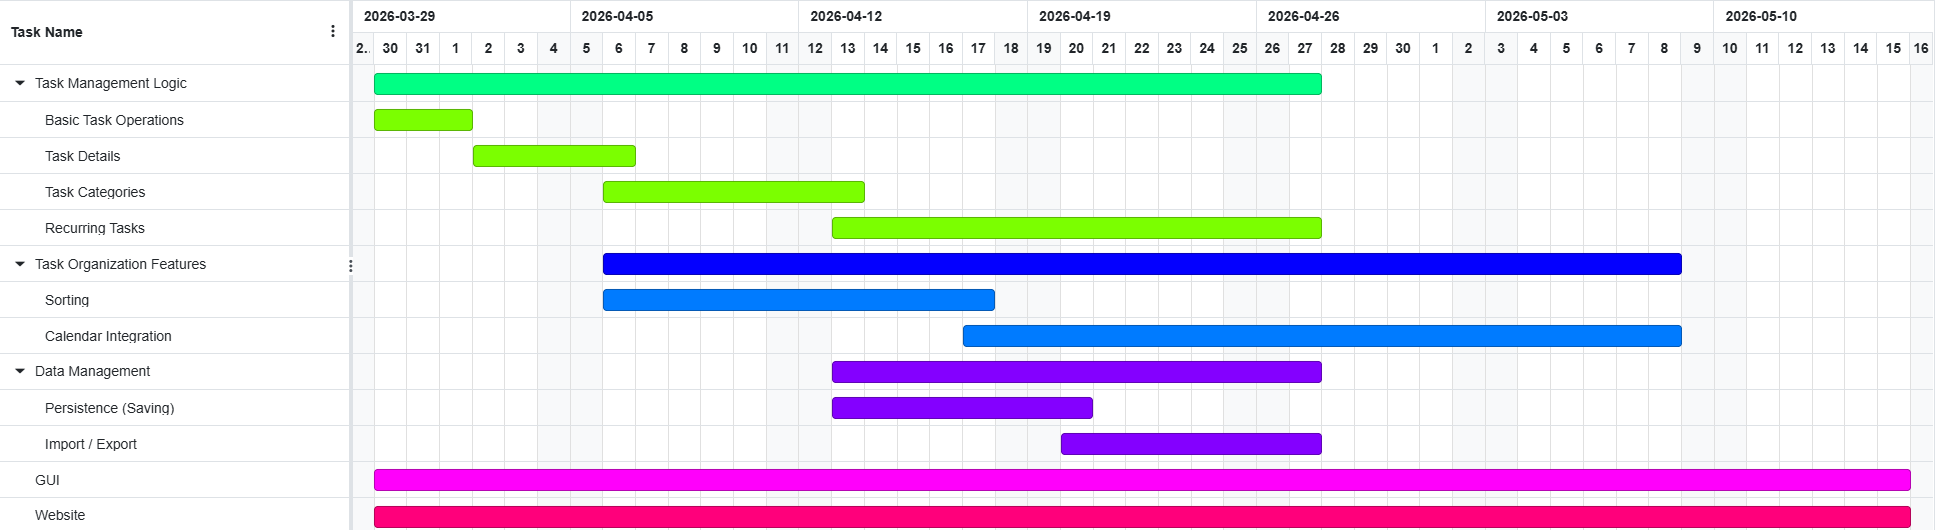
\includegraphics[width=9in, angle=90]{illustrations/gantt_diagram.png}
\end{figure}

Seven weeks make up the timeline, running late March into May. Because of how the global student swap lined up, that window was the only option available. So narrowing down what mattered most became unavoidable. Key parts of the software took center stage instead of extras. Picking each step with care kept things moving without delays. Time pressed close, yet choices stayed sharp.
\\

By mid-May comes the last defense, setting the stage for what began earlier: building a base strong enough to hold everything else. Starting that effort meant shaping how the task manager would work at its root level. The way tasks connect, through details like name, condition, rank, and deadline, had to be mapped out carefully. From there, basic actions took shape: making tasks appear, letting them change, allowing removal, keeping them saved using files on disk.
\\

Right away, steady task management took center stage because shaky operations would weaken everything else. Data staying accurate mattered just as much since trust in the app depends on it. The setup branched out cleanly so additions later, like sorting or tighter grouping, would fit without chaos. Design choices leaned toward growth, meaning new features can slip in without tearing things apart.
\\

Later on, new pieces got added while moving toward the last review. Features like sorting by urgency came in, along with systems to follow progress and handle tricky dates - especially those that repeat every month. Instead of clutter, a cleaner layout took shape so people could see tasks better and work with them more naturally.
\\

Those final stretch leading up to the mid-May presentation focused on checking everything, fixing errors, then smoothing out rough edges so all parts worked together without hiccups. Getting a working order into place for handling tasks in just seven weeks shows what clear goals, group effort, and smart scheduling can do when time runs short.

\subsubsection{Task distribution}
\begin{table}[h!]
    \centering
    \begin{tabular}{|l|l|}
        \hline
        \textbf{Task} & \textbf{Responsible}\\
        \hline
        Basic Task Operation & Adrien\\
        \hline
        Task Details & Adrien\\
        \hline
        Task Categories & Alexandre\\
        \hline
        Reccurring Task & Quentin\\
        \hline
        Sorting & Quentin\\
        \hline
        Calendar Integration & Jérôme\\
        \hline
        Persistence (Saving) & Alexandre\\
        \hline
        Import/Export & Alexandre\\
        \hline
        GUI & Jérôme\\
        \hline
        Website & Adrien\\
        \hline
    \end{tabular}
\end{table}


\subsubsection{Actual progress of the project}
The Task List project reached completion on time, even though deadlines pressed hard. Though tight, the schedule did not block progress, every core function made it into the build. Requirements laid out early held firm throughout development; functionality matched what was asked. Management tools work as needed, structure stays clear, information saves reliably. Each goal from the spec document now exists in practice, no gaps left behind.





\newpage
\section{Specific tasks explanation}
In this part of the document, each task will be presented in order to better understand choices of implementation that were made by the team, the challenges that were faced and the technological tools used. 

\subsection{Basic Task Operation}
The implementation of tasks within the Rust application was carried out through the definition of a structured data model representing each task as an instance of a Task entity. Each task is initialized using a dedicated constructor function, which assigns default and user-defined values to its attributes. The new function was designed to take as input the task name, description, category identifier, priority level, optional due date, and recurrence configuration. During instantiation, the task is assigned a default identifier value of zero and an initial status set to pending, ensuring that all newly created tasks begin in a consistent state before being processed or stored within the system.
\\

In addition to task creation, utility methods were implemented to handle task-related data formatting and access. In particular, a method was defined to retrieve the due date of a task in a standardized string format. This method accounts for the optional nature of the due date field by verifying its presence. When a date exists, it is formatted according to a year-month-day pattern; otherwise, an empty string is returned. This design choice ensures robustness by preventing invalid date access while maintaining a consistent output format for display and processing purposes.
\\

The priority system was also explicitly defined using an enumerated structure representing the different levels of task importance. A static collection containing all possible priority values was implemented to facilitate iteration and validation across the system. This approach ensures that priority handling remains centralized and consistent, ranging from non-prioritized tasks to critical-level tasks. By defining this fixed set of values, the system guarantees strict control over allowed priority states, reducing ambiguity and improving maintainability of the task management logic.



\subsection{Task Details}
The implementation of task-related operations was extended through the definition of additional behaviors that allow the system to manipulate and interpret task data efficiently. Beyond the creation and initialization of tasks, specific attention was given to how task attributes are accessed and processed during runtime. This includes the handling of optional fields and the standardization of output formats in order to ensure consistent behavior across the application.
\\

In particular, utility methods were introduced to manage task metadata in a safe and structured manner. The retrieval of the due date is handled through a dedicated function that checks the existence of a value before attempting any formatting operation. This approach prevents invalid access to optional data and ensures that the system remains robust even when certain attributes are not defined. When a due date is present, it is converted into a standardized string representation, ensuring uniformity across all task displays and interactions. In the absence of a defined date, an empty value is returned to preserve predictable system behavior.
\\

Furthermore, the priority system plays a central role in task classification and filtering. It is implemented as a fixed enumerated type defining all possible priority levels supported by the application. This enumeration is complemented by a static collection containing all valid priority values, which facilitates iteration, validation, and comparison operations throughout the system. By explicitly defining the full set of priority states, the implementation ensures strong type safety and prevents invalid or inconsistent priority assignments.
\\

Overall, these design choices contribute to a coherent and reliable task management system in which task creation, attribute handling, and priority classification are tightly controlled and consistently enforced across the application logic.



\subsection{Task Categories}

To help organize data, the system includes a categorization feature that allows users to effectively group, identify, and filter their tasks.
\\

Each category is represented by the Category structure, which contains two main attributes: a unique ID and a name. All categories are managed centrally using the CategoryList structure, which holds a dynamic vector. 
\\

When adding a new category, the system automatically assigns an ID. It starts the ID at 1 and increases it dynamically by checking the IDs already present in the list. This approach ensures a reliable identification of categories without requiring any action from the user or complex dependencies. As a result, the user can select different categories when creating a new task.
\\
\begin{figure}[H]
    \centering
    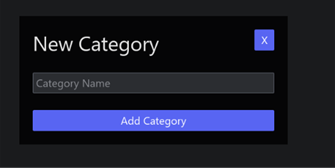
\includegraphics[width=2in]{illustrations/categories/new.png}
    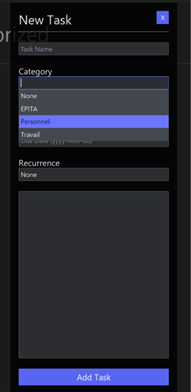
\includegraphics[width=2in]{illustrations/categories/change.png}
\end{figure}

Finally, the system offers flexible management, allowing the user to easily rename or delete existing categories. 
\\
\begin{figure}[H]
    \centering
    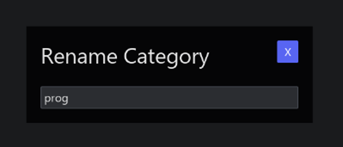
\includegraphics[width=2in]{illustrations/categories/rename.png}
\end{figure}



\subsection{Recurring Task}
The implementation of the recurring tasks system is one of the project's most important features. In a task management application, many actions need to be repeated on a regular basis, such as weekly meetings, monthly payments, daily workouts, or certain administrative tasks. The goal of this feature was therefore to allow users to automate the creation of these recurring tasks to improve the app's overall efficiency and usability.
\\

Before this feature was implemented, each task had to be manually recreated after it was completed. This approach had several limitations, including wasted time for the user and a significant risk of forgetting tasks. The recurrence system we developed now automatically generates a new instance of a task when it is marked as completed.
\\

From a technical standpoint, this feature required a modification to the main structure representing tasks in the application. Additional information related to the recurrence frequency was added to define the behavior of each recurring task. The project supports several types of recurrence, including daily, weekly, and monthly recurrences. The Rust programming language allowed us to represent these different cases robustly using enumerations (enums), which ensures greater program safety and reduces the risk of errors related to invalid values.
\\

When a recurring task is confirmed by the user, the program automatically triggers a mechanism to generate a new task. This new instance retains the essential information from the original task, such as its title or category, but its due date is recalculated based on the selected frequency. For example, a daily task will be automatically recreated for the following day, while a weekly task will be moved to the following week.
\\

Date management represented a particularly important part of the development process. Indeed, the automatic calculation of deadlines can become complex depending on the situations encountered. Some months have a different number of days, and certain calendar transitions require specific adjustments. To ensure data consistency, several validation checks were implemented during the generation of new occurrences.
\\

This feature brings real added value to the final project, as it makes the application closer to the standards found in professional productivity management tools. It significantly improves user experience by reducing repetitive actions and automating an important part of daily organization.
\begin{figure}[H]
    \centering
    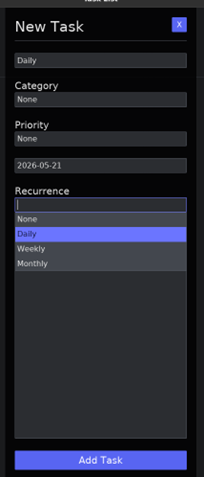
\includegraphics[width=2in]{illustrations/recurring/set.png}
    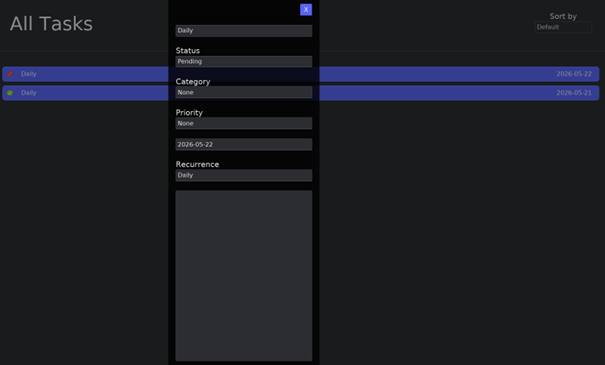
\includegraphics[width=5in]{illustrations/recurring/application.png}
\end{figure}



\newpage
\subsection{Sorting}
The task sorting and organization system is a key feature of the project, as it directly improves the readability and management of the information displayed in the application. In a task manager, an increase in the number of items can quickly make the interface difficult to use if no sorting mechanism is in place. The main objective of this feature was therefore to allow users to efficiently organize their tasks according to various criteria.
\\

Several sorting methods were developed within the app to provide a smoother and more intuitive navigation experience. Tasks can be sorted by due date, alphabetical order, progress status, or priority. This system makes it possible to quickly identify urgent tasks, tasks that have already been completed, or those requiring special attention.
\\

Implementing categories required adding new relationships between the project's various data structures. Each task must maintain a consistent reference to its category, even after sorting, modification, or deletion. This part of the development required special attention to avoid data inconsistencies and maintain good performance.
\\

Developing this feature also provided an opportunity to delve deeper into several key concepts of the Rust programming language, including collection manipulation, custom comparisons, and memory management mechanisms. While the constraints imposed by the Rust compiler sometimes made certain implementations more complex, they also helped enhance the program's overall reliability.
\\

Thanks to this sorting and categorization system, the application has become more user-friendly and better suited for real-world use. These features significantly enhance the user experience and provide a solid foundation for potential future developments, such as the addition of advanced filters, a search engine, or a more dynamic graphical interface.
\begin{figure}[H]
    \centering
    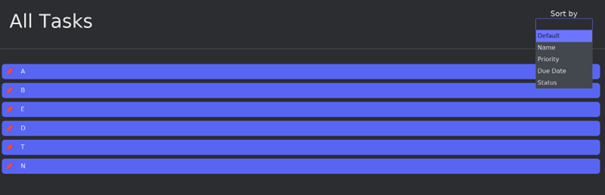
\includegraphics[width=5in]{illustrations/sorting/default.png}
    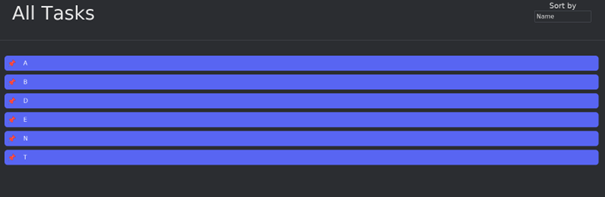
\includegraphics[width=5in]{illustrations/sorting/name.png}
    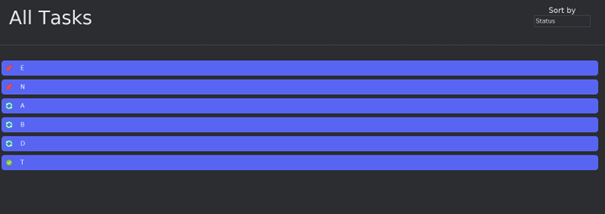
\includegraphics[width=5in]{illustrations/sorting/status.png}
\end{figure}



\subsection{Calendar Integration}
\paragraph{Custom Interface Implementation}\hfill

The calendar integration is a core component of the graphical user interface, designed to provide a standard monthly grid view where each row represents a week. Because the Iced library lacks a native, pre-built calendar widget, a custom solution was engineered. This implementation leverages Iced's fundamental layout primitives—specifically rows and columns. Individual days are encapsulated within container widgets and visually delineated by borders, resulting in a clean, structured calendar grid.

\paragraph{Task Visualization and Interaction}\hfill

Within each day's container, the application renders a vertical list of tasks scheduled for that specific date. To effectively manage GUI real estate and accommodate days with a high volume of activities, these task lists are embedded within scrollable viewports. Furthermore, each listed task functions as an interactive element. Users can click on any task button within the calendar to seamlessly access and modify its specific fields and attributes.

\paragraph{Temporal Logic and Navigation}\hfill

To handle the underlying date and time logic, the application integrates the chrono library. This crate is utilized to accurately compute the structural matrix of each month, specifically calculating the dynamic number of weeks required for the grid layout (which naturally fluctuates between five and six weeks depending on the month and year). This logic ensures a precise and visually consistent calendar rendering. Finally, temporal navigation controls were implemented, enabling users to fluidly transition between the current, previous, and subsequent months.
\begin{figure}[H]
    \centering
    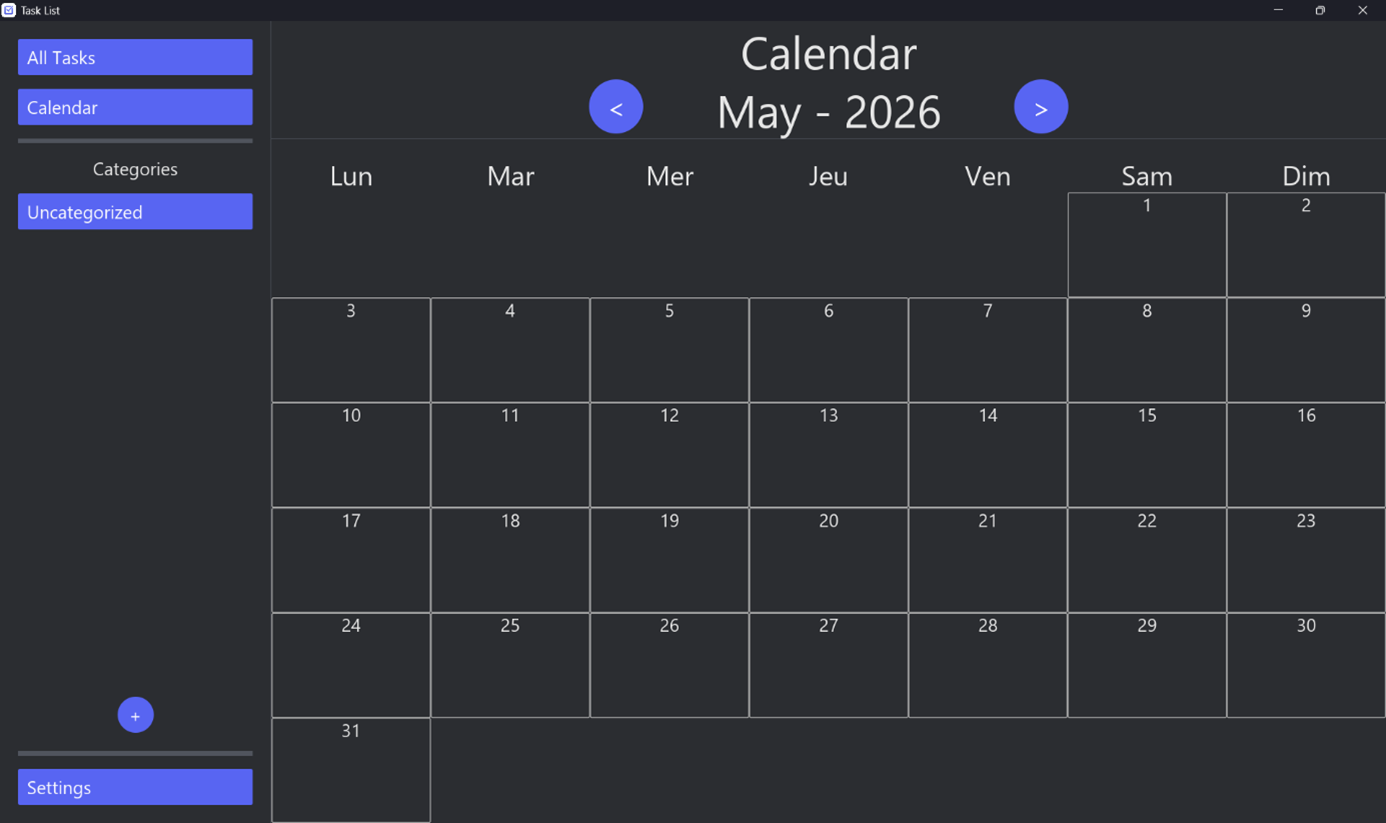
\includegraphics[width=5in]{illustrations/calendar/CalendarView.png}
    \caption*{Calendar View}
\end{figure}



\subsection{Persistence}
To ensure a good user experience, it was essential for the application to save and restore data between sessions without any alteration or loss of information. The persistence system was designed around a simple and robust approach, relying on the standardized JSON format. 
\\

To centralize the application's state management, a structure named SaveData was implemented. This structure groups the task list and the category list into a single serializable unit. This design choice simplifies saving and loading operations by treating the entire application state as a single object, rather than managing multiple separate files. Using this unified structure allows read and write operations to be performed in a single pass.
\\

The data conversion process relies heavily on the serde library and its serde\_json module, which are standards in the Rust ecosystem for converting data structures to and from JSON. The choice of JSON as the storage format was deliberate because it is readable, easy to debug, and well-suited for import/export. The data is written with an indented formatting (pretty-print), making the output file easy for the user to inspect and modify if necessary.
\\

The save function serializes the current SaveData instance and writes it directly to a specified file path. The load function handles several edge cases to ensure the system's robustness because if the target file does not exist, or if it is empty, the function simply returns an empty SaveData object instead of throwing an error. This makes the application's first launch completely transparent, requiring no prior configuration from the user.
\\

One of the main challenges of this module was ensuring that data integrity was maintained across all possible application states, especially after sorting, modifying, or deleting tasks. Since the save operation captures the complete state at a given moment, it was crucial for other modules to maintain consistent internal representations before triggering a save.
\\

Users can manually save their data from the Settings tab. More importantly, this system keeps the app reliable by automatically saving after every change whether users add, edit, delete, or sort a task. This guarantees that no data is ever lost between sessions.

\subsection{Import/Export}
The import/export feature allows the user to save their data outside the application or restore it from an external file. It is accessible from the Settings tab in the user interface.
\\

The export operation prompts the user to select a destination folder using the operating system's native file explorer. Once a folder is chosen, the app's current state is saved first. Then, the save.json file is copied to the selected folder and renamed as task-list\_data.json. This allows the user to keep a backup of their data anywhere they want, which is useful for safe-keeping or transferring it to another computer.

\begin{figure}[H]
    \centering
    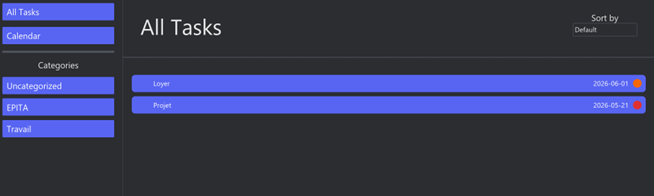
\includegraphics[width=5in]{illustrations/import-export/data.png}
    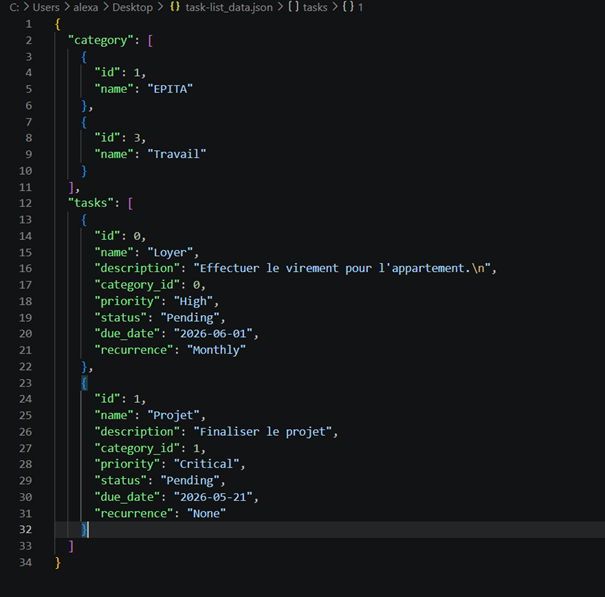
\includegraphics[width=5in]{illustrations/import-export/json.png}
\end{figure}

The import operation works the other way around: file selection window, filtered to show only JSON files, lets the user select a data file. The application starts by resetting its current state. It then copies the selected file to the internal save file location and reloads all tasks and categories. Finally, the lists are resorted, and the interface components are updated accordingly, especially the category dropdown menu.

\subsection{GUI}
\paragraph{Technology Stack Selection}\hfill

During the initial design phase, the Tauri framework was considered for the application's GUI. While Tauri is highly capable, utilizing an HTML, CSS, and JavaScript frontend alongside a Rust backend, this approach was ultimately discarded. Adopting Tauri would have shifted the project paradigm too closely toward web development rather than maintaining a pure, native Rust application.
\\

Consequently, the decision was made to adopt Iced (version 0.14.0), a robust GUI library written entirely in Rust. This framework was selected for its native Rust ecosystem integration and its excellent cross-platform compatibility, ensuring seamless execution on both Windows and Linux operating systems.

\paragraph{Architectural Design}\hfill

The application's architecture follows Iced's Elm-inspired design pattern, which systematically separates logic and presentation into three primary components:
\begin{itemize}
    \item \textbf{new:} Acts as the entry point, initializing the application's core structure and default state.
    \item \textbf{update:} Processes incoming user interactions (messages) and executes the corresponding state transitions or actions.
    \item \textbf{view:} Renders the current state of the GUI to the user. 
\end{itemize}

\begin{figure}[H]
    \centering
    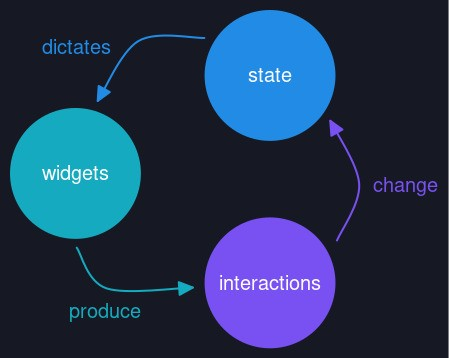
\includegraphics[width=3in]{illustrations/gui/ArchitecturalDesign.jpg}
    \caption*{Architecture}
\end{figure}

\paragraph{User Interface Layout and Navigation}\hfill

The view implementation utilizes intuitive UI primitives—such as text, buttons, rules, spaces, text inputs, and comboboxes. Layout management is handled efficiently using rows, columns, and containers. This results in a clean, minimalist, and highly readable interface.
\\

The main screen features a split-layout design, utilizing a persistent sidebar for navigation between the following core tabs:
\begin{itemize}
    \item \textbf{All Tasks:} A comprehensive list displaying all user tasks.
    \item \textbf{Calendar:} A chronological, calendar-based view of upcoming tasks.
    \item \textbf{Categories:} Dynamic tabs corresponding to user-defined categories, filtering tasks by their specific classification.
    \item \textbf{Settings:} A configuration hub allowing users to save, export, and import their data, as well as reset the application state.
\end{itemize}

\begin{figure}[H]
    \centering
    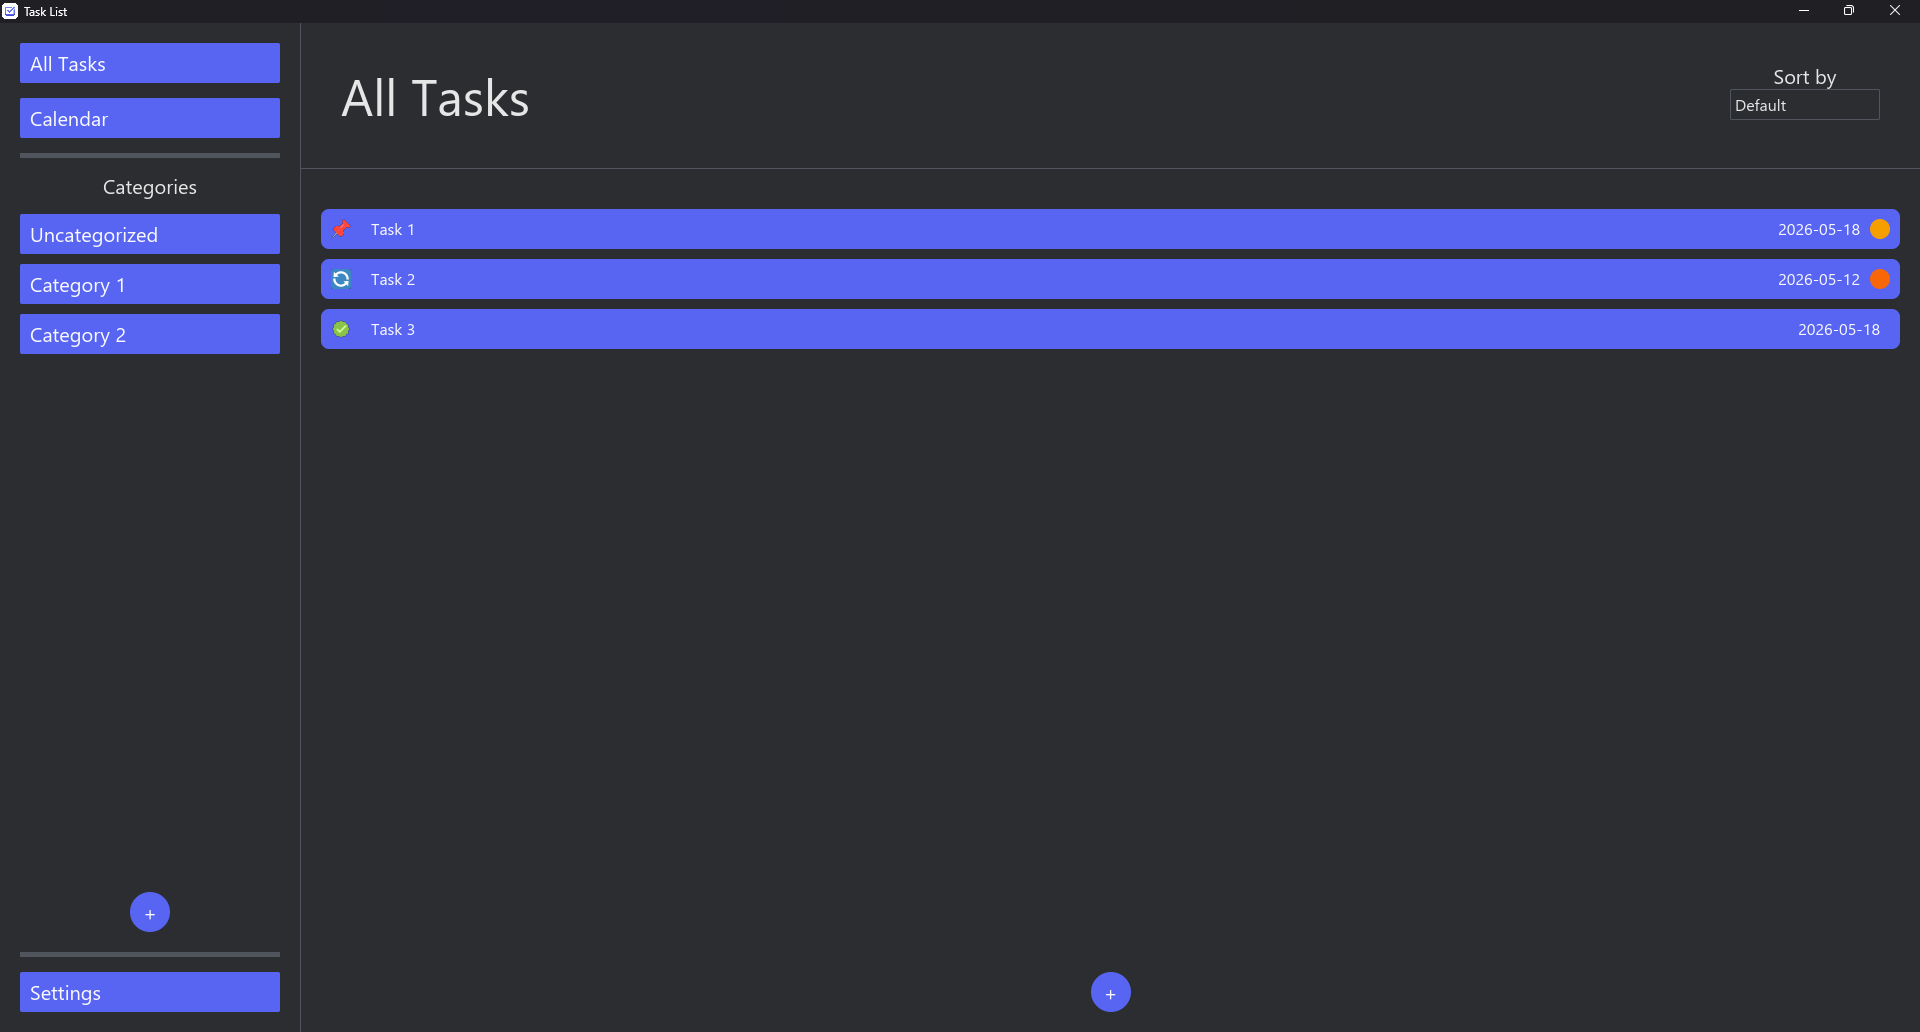
\includegraphics[width=5in]{illustrations/gui/AlltaskTab.png}
    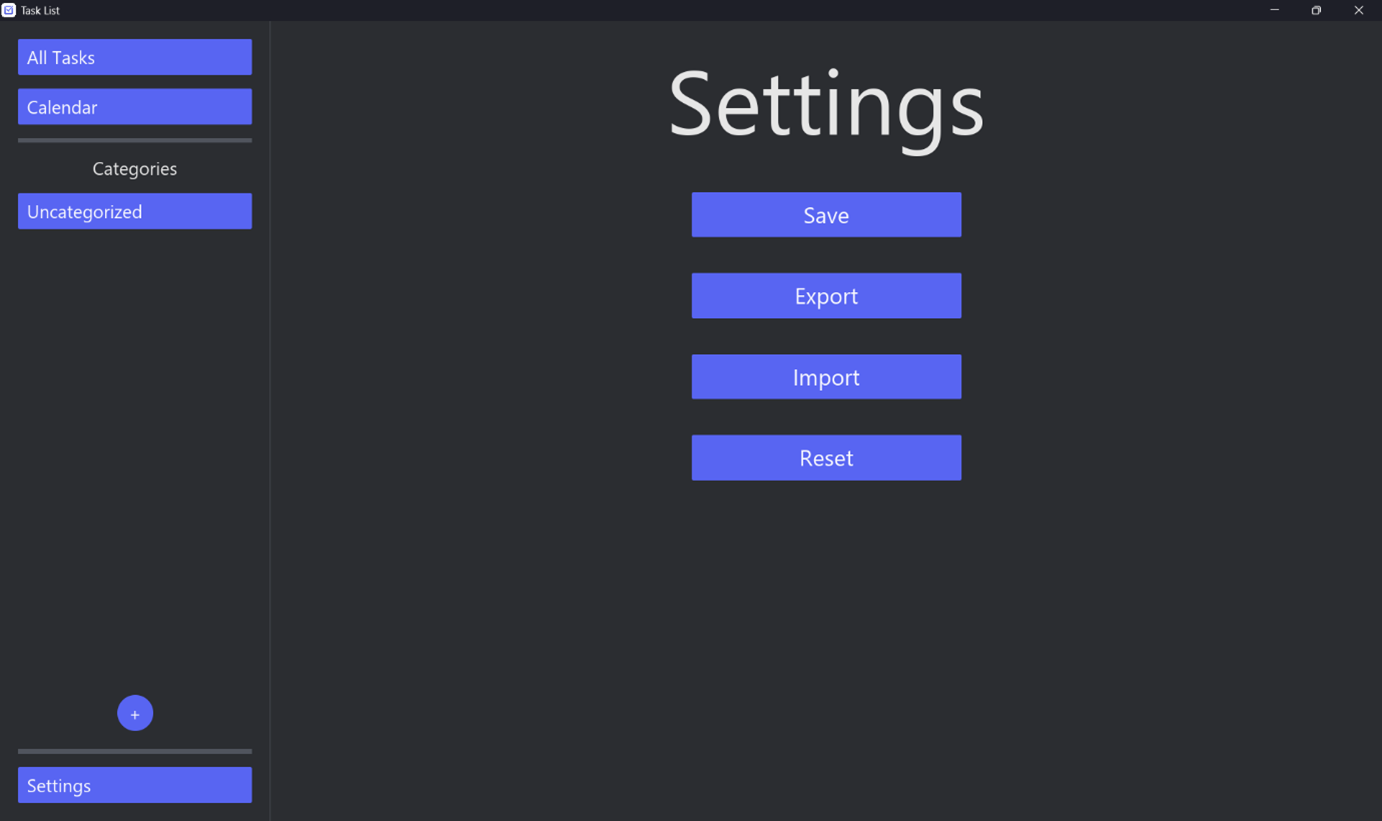
\includegraphics[width=5in]{illustrations/gui/SettingsTab.png}
    \caption*{All Task \& Settings Tab}
\end{figure}

\paragraph{Component Design and Modals}\hfill

To ensure a smooth user experience, dynamic components were carefully integrated. Text inputs are utilized for defining task attributes and category names. Comboboxes are employed for managing task states, priorities, and sorting mechanisms, significantly enhancing overall usability. To gracefully handle extensive data, scrollable viewports were implemented for both the main task list and the sidebar category list, ensuring usability when the number of items exceeds the window dimensions.
\\

For modal interfaces (popups), Iced's Stack widget was utilized to overlay UI elements securely on top of the main application. To provide clear visual feedback and prevent unintended interactions, a semi-transparent, opaque gray background is rendered behind the active popup, intuitively signaling to the user that the underlying application layers are temporarily disabled.
\begin{figure}[H]
    \centering
    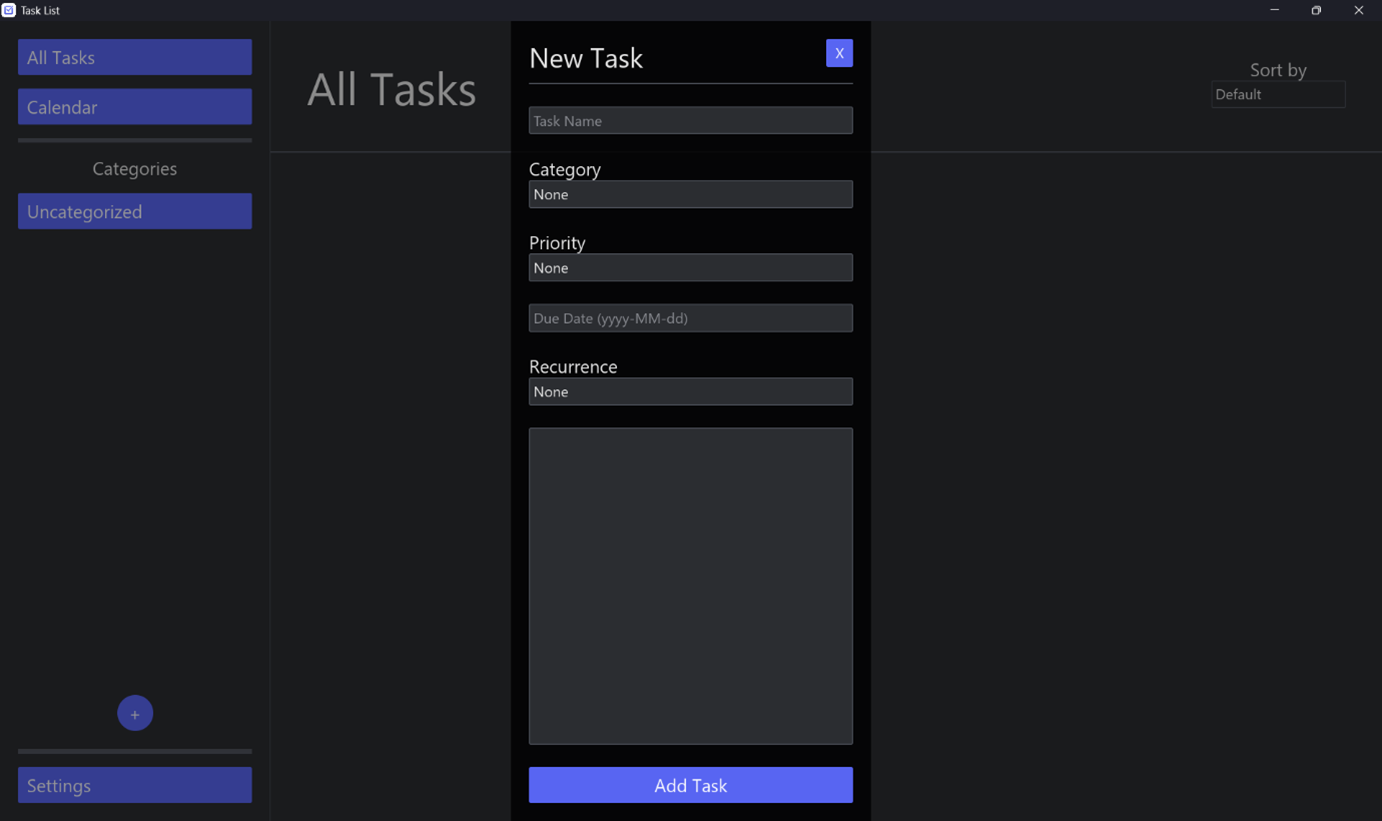
\includegraphics[width=5in]{illustrations/gui/Popup.png}
    \caption*{New Task Popup}
\end{figure}

\paragraph{Data Management and Native Dialogs}\hfill

To facilitate the import and export of user data from the "Settings" tab, the application integrates the rfd (Rust File Dialog) crate. When a user initiates an export or import action, rfd triggers the operating system's native file explorer dialog, allowing the user to seamlessly select the desired file path.



\subsection{Website}
As part of the Task-List project, a software application developed in Rust, a dedicated documentation website was designed and implemented to present and explain the features of the system. The primary objective of this website is to provide a clear, structured, and accessible documentation layer that enables users and developers to understand the application without directly inspecting the source code. The website serves as a static informational interface built using standard web technologies, namely HTML, CSS, and JavaScript, and is deployed using GitHub Pages to ensure simple and public accessibility.
\\

The main purpose of the documentation website is to offer a comprehensive presentation of the Task-List application while maintaining clarity and simplicity. The website was designed to structure both functional and technical information in a readable format, making it easier for users to navigate through the different aspects of the project. It also aims to separate the core logic implemented in Rust from the documentation layer, ensuring a clear distinction between backend functionality and user-facing explanation. Finally, the website was intended to be lightweight, easily maintainable, and fully accessible online without requiring any server-side infrastructure.
\\

This project demonstrates the successful design and implementation of a static documentation website for a Rust-based application. It highlights the ability to structure technical information clearly and to present a software project through an accessible web interface. The use of HTML, CSS, and JavaScript without frameworks allowed for full control over the design and structure of the site while maintaining simplicity and performance.
\\

Overall, the website effectively fulfills its role as a documentation layer for the Task-List application. It improves the accessibility of the project, provides a clear explanation of its functionalities, and enhances its presentation as a complete software system. It also enables a form of project tracking by centralizing information about the application’s structure, features, and evolution in a single and consistent interface. Future improvements could include the addition of a dark mode, a search functionality within the documentation, or even automatic generation of documentation directly from the Rust source code.





\section{Bibliography}
For this Task List project, the team used several resources listed below.
\begin{itemize}
    \item Documentation of Iced 0.14.0 \url{Website}
\end{itemize}





\newpage
\section{Conclusion}
To conclude, the Task List team has been pleased to work on this project. It has been a valuable experience for all members of the group. Developing a task management application allowed the team to strengthen both their technical skills, particularly in software design and data management, as well as their organizational and communication abilities, which were essential to work effectively within a limited timeframe.

\end{document}